\section{Preliminaries}\label{sec:preliminiary}

Polkadot was first introduced in 2016 by Gavin Wood \cite{2016:Wood:Polkadot} that presented Polkadot's preliminary roles as follows. 

Polkadot network consists of a large number of validatable, globally-coherent dynamic “parallelised” data-structures called  \emph{parachains} and the bedrock upon which those parachains are interacting, are known as \emph{the relay chains}. Figure \ref{fig:roles} shows these subcomponents alongside the sub-actors of the system which are in play to deliver the Polkadot scalable heterogeneous multi-chain system.

\begin{figure}[h]
	\centering
	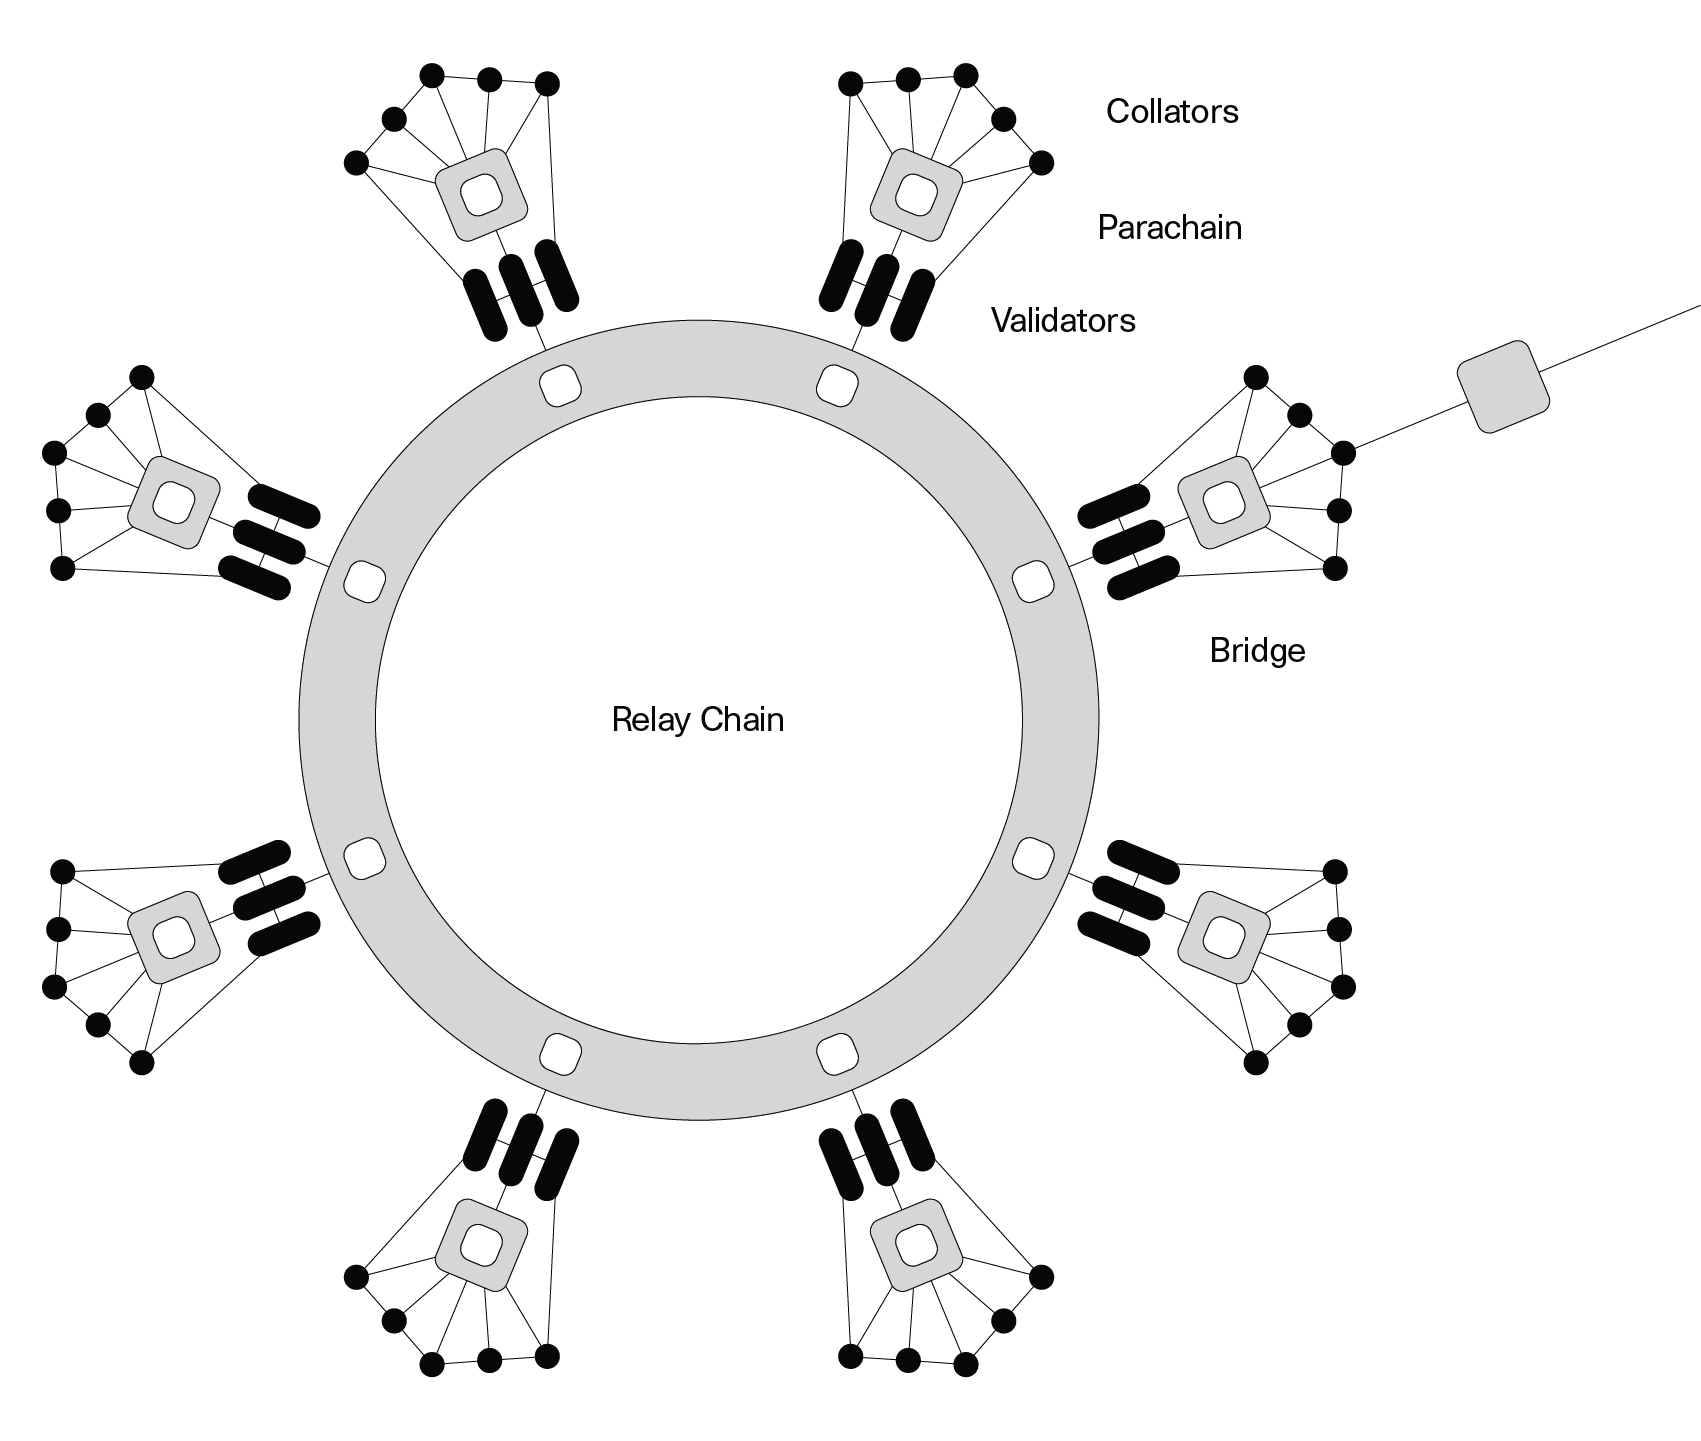
\includegraphics[width=.7\textwidth]{images/Network@2x.png}
	\caption{Polkadot network structure showing relay chain and parachain and including the roles collator, validator (Image credit: Ignasio Albero)}
	\label{fig:roles}
\end{figure}
\subsection{Structural elements of Polkadot}

Polkadot is a scalable heterogeneous multi-chain. This means that unlike previous blockchain implementations which have focused on providing a single chain of varying degrees of generality over potential applications, Polkadot itself is designed to provide no inherent application functionality at all. Rather, Polkadot provides the bedrock “relay-chain” upon which a large number of validatable, globally-coherent dynamic data-structures may be hosted side-by-side.
We call these data-structures “parallelised” chains or parachains, though there is no specific need for them to be blockchain in nature.
In other words, Polkadot may be considered equivalent to a set of independent chains (e.g. the set containing Ethereum, Ethereum Classic, Namecoin and Bitcoin) except for two very important points:
\begin{itemize}
\item Pooled security;
\item trust-free interchain transactability.
\end{itemize}
These points are why we consider Polkadot to be “scalable”. In principle, a problem to be deployed on Polka- dot may be substantially parallelised—scaled out—over a large number of parachains. Since all aspects of each parachain may be conducted in parallel by a different segment of the Polkadot network, the system has some ability to scale. Polkadot provides a rather bare-bones piece of infrastructure leaving much of the complexity to be ad- dressed at the middleware level. This is a conscious decision intended to reduce development risk, enabling the requisite software to be developed within a short time span and with a good level of confidence over its security and robustness.

The structural elements and different roles defined in the Polkadot protocol and, as shown in Figure~\ref{fig:roles}.

\syed{}{perhaps we should use more technical language in this section. I'll try to do so in my review.}

%\paragraph{Chain} (or a blockchain) broadly refers to a state machine which possibly replicated in a decentralized environment. By a block we refer to a recorded list of transactions which have been applied to change the state of a chain.


%\paragraph{Relay Chain:} is the Polkadot central state machine which keeps references to the current states of all parachains and to the cross parachain transactions. Thus the relay chain works as a single source of truth across Polkadot network.
%\syed{It also keeps references of all cross-parachain messages}{-remove- mentioned above as cross parachain transaction, what is a message otherwise? we need to define it first}.

\subsection{Roles}
Nodes which run Polkadot network assume different roles to ensure the properties introduced in Section \ref{sec:properties}. In the following, we introduce these roles and their functions.

%I'm looking at the definition of these roles in the original paper and in many case they look more comprehensive than what we have here. Perhaps, we could incorporate more of the original white paper here.
  
\paragraph{Validators:} A validator is the highest charge and helps seal new blocks on the Polkadot network. The validator’s role is contingent upon a sufficiently high bond being deposited, though we allow other bonded parties to nominate one or more validators to act for them and as such some portion of the validator’s bond may not necessarily be owned by the validator itself but rather by these nominators.
A validator must run a relay-chain client implementation with high availability and bandwidth. At each block the node must be ready to accept the role of ratifying a new block on a nominated parachain. This process involves receiving, validating and republishing candidate blocks. The nomination is deterministic but virtually un- predictable much in advance. Since the validator cannot reasonably be expected to maintain a fully-synchronised database of all parachains, it is expected that the validator will nominate the task of devising a suggested new parachain block to a third-party, known as a collator.
Once all new parachain blocks have been properly ratified by their appointed validator subgroups, validators must then ratify the relay-chain block itself. This involves updating the state of the transaction queues (essentially moving data from a parachain’s output queue to another parachain’s input queue), processing the transactions of the ratified relay-chain transaction set and ratifying the final block, including the final parachain changes. A validator not fulfilling their duty to find consensus under the rules of our chosen consensus algorithm is punished. For initial, unintentional failures, this is through withholding the validator’s reward. Repeated failures re- sult in the reduction of their security bond (through burn- ing). Provably malicious actions such as double-signing or conspiring to provide an invalid block result in the loss of the entire bond (which is partially burnt but mostly given to the informant and the honest actors).
In some sense, validators are similar to the mining pools of current PoW blockchains.

\paragraph{Nominators:} "A nominator is a stake-holding party who contributes to the security bond of a validator. They have no additional role except to place risk capital and as such to signal that they trust a particular validator (or set thereof) to act responsibly in their maintenance of the network. They receive a pro-rata increase or reduction in their deposit according to the bond’s growth to which they contribute.
Together with collators, next, nominators are in some sense similar to the miners of the present-day PoW net- works."

\paragraph{Collators: } Transaction collators (collators for short) are parties who assist validators in producing valid parachain blocks. They maintain a “full-node” for a particular parachain; meaning that they retain all necessary information to be able to author new blocks and execute transactions in much the same way as miners do on cur- rent PoW blockchains. Under normal circumstances, they will collate and execute transactions to create an unsealed block, and provide it, together with a zero-knowledge proof, to one or more validators presently responsible for proposing a parachain block.
The precise nature of the relationship between collators, nominators and validators will likely change over time. Initially, we expect collators to work very closely with validators, since there will be only a few (perhaps only one) parachain(s) with little transaction volume. The initial client implementation will include RPCs to allow a parachain collator node to unconditionally supply a (relay- chain) validator node with a provably valid parachain block. As the cost of maintaining a synced version of all such parachains increases, we expect to see additional infrastructure in place which will help separate out the duties to independent, economically-motivated, parties.
Eventually, we expect to see collator pools who vie to collect the most transaction fees. Such collators may be- come contracted to serve particular validators over a period of time for an on-going share in the reward proceeds. Alternatively, “freelance” collators may simply create a market offering valid parachain blocks in return for a competitive share of the reward payable immediately. Similarly, decentralised nominator pools would allow multiple bonded participants to coordinate and share the duty of a validator. This ability to pool ensures open participation leading to a more decentralised system.

\paragraph{Fishermen:} Unlike the other two active parties, fishermen are not directly related to the block-authoring process. Rather they are independent “bounty hunters” motivated by a large one-off reward. Precisely due to
the existence of fishermen, we expect events of misbehaviour to happen seldom, and when they do only due to the bonded party being careless with secret key security, rather than through malicious intent. The name comes from the expected frequency of reward, the minimal requirements to take part and the eventual reward size.
Fishermen get their reward through a timely proof that at least one bonded party acted illegally. Illegal actions include signing two blocks each with the same ratified par- ent or, in the case of parachains, helping ratify an invalid block. To prevent over-rewarding or the compromise and illicit use of a session’s secret key, the base reward for providing a single validator’s illegally signed message is minimal. This reward increases asymptotically as more corroborating illegal signatures from other validators are provided implying a genuine attack. The asymptote is set at 66$\%$ following our base security assertion that at least two-thirds of the validators act benevolently.
Fishermen are somewhat similar to “full nodes” in present-day blockchain systems that the resources needed are relatively small and the commitment of stable uptime and bandwidth is not necessary. Fishermen differ in so much as they must post a small bond. This bond prevents sybil attacks from wasting validators’ time and compute resources. It is immediately withdrawable, probably no more than the equivalent of a few dollars and may lead to reaping a hefty reward from spotting a misbehaving validator.

\subsection{Adversarial Model of Polkadot}

%The adversarial assumption on collators depends on the parachain type. If the parachain is private,
%we assume that there is at least one honest collator.
%Otherwise, we assume that at least the majority of collators are honest.
\paragraph{Roles:} In general, we assume that honest parties follow the protocol while malicious ones can follow any arbitrary algorithm. We assume that three quarters of nominators' stake belong to honest ones. As a result of this assumption, more than two third of validators who are elected by nominators are honest. We do not have any limit on number of malicious fishermen since their malicious behaviours are detectable and punishable.  

\paragraph{Parachains:} We do not have any security assumption on block production mechanism of parachain. On the other hand, we assume that a significant amount of collators are honest. The security of Polkadot does not depend on any precise honest fraction of collators but it requires existence of some honest collators.

\paragraph{Keys:} We assume that malicious parties generate their keys with an arbitrary algorithm
while honest ones always generate their keys securely. 

\paragraph{Network and Communication:} All validators have their own local clock and their clocks do not rely on any central clock.
We assume that  validators and collators are in a partially synchronous network.
It means that a message sent by a validator or collator arrives at all parties in the network
at most $\D$ units of time later where $\D$ is an unknown parameter. So, we assume an eventual delivery of a message in Polkadot.
We also assume that collators and fishermen can connect to the relay chain network to submit their reports.
%TODO: Do we have authenticated channel between validators?


